% EffectShield project report (DEL-03). Build: tectonic docs/report/effectshield_report.tex
% Result numbers come from generated/results.tex (scripts/report_tables.py), never typed by hand.
\documentclass[11pt]{article}
\usepackage[margin=1in]{geometry}
\usepackage[T1]{fontenc}
\usepackage{lmodern}
\usepackage{microtype}
\usepackage{amsmath,amssymb}
\usepackage{booktabs}
\usepackage{tabularx}
\usepackage{array}
\usepackage{xcolor}
\usepackage{tikz}
\usetikzlibrary{arrows.meta,positioning,fit,calc,shapes.geometric}
\usepackage{caption}
\usepackage{enumitem}
\usepackage[hidelinks]{hyperref}
\setlist{nosep,leftmargin=1.4em}
\setlength{\emergencystretch}{2em}
\captionsetup{font=small,labelfont=bf}
\definecolor{esblue}{HTML}{2A78D6}
\definecolor{uporange}{HTML}{EB6834}
\definecolor{spaqua}{HTML}{1BAF7A}
\definecolor{muted}{HTML}{52514E}
% Generated by scripts/report_tables.py from retained evidence. Do not edit.
\newcommand{\rateESattackedunsafeeffect}{0.0}
\newcommand{\loESattackedunsafeeffect}{0.0}
\newcommand{\hiESattackedunsafeeffect}{0.0}
\newcommand{\nESattackedunsafeeffect}{0/56}
\newcommand{\rateUPattackedunsafeeffect}{58.3}
\newcommand{\loUPattackedunsafeeffect}{38.9}
\newcommand{\hiUPattackedunsafeeffect}{76.4}
\newcommand{\nUPattackedunsafeeffect}{30/56}
\newcommand{\rateSPattackedunsafeeffect}{45.8}
\newcommand{\loSPattackedunsafeeffect}{25.0}
\newcommand{\hiSPattackedunsafeeffect}{66.7}
\newcommand{\nSPattackedunsafeeffect}{24/56}
\newcommand{\rateESattacksuccess}{6.2}
\newcommand{\loESattacksuccess}{0.0}
\newcommand{\hiESattacksuccess}{16.7}
\newcommand{\nESattacksuccess}{3/56}
\newcommand{\rateUPattacksuccess}{64.6}
\newcommand{\loUPattacksuccess}{45.8}
\newcommand{\hiUPattacksuccess}{81.9}
\newcommand{\nUPattacksuccess}{33/56}
\newcommand{\rateSPattacksuccess}{50.0}
\newcommand{\loSPattacksuccess}{29.2}
\newcommand{\hiSPattacksuccess}{70.8}
\newcommand{\nSPattacksuccess}{25/56}
\newcommand{\rateEScleancompletion}{98.6}
\newcommand{\loEScleancompletion}{95.8}
\newcommand{\hiEScleancompletion}{100.0}
\newcommand{\nEScleancompletion}{55/56}
\newcommand{\rateUPcleancompletion}{70.8}
\newcommand{\loUPcleancompletion}{54.2}
\newcommand{\hiUPcleancompletion}{87.5}
\newcommand{\nUPcleancompletion}{40/55}
\newcommand{\rateSPcleancompletion}{70.8}
\newcommand{\loSPcleancompletion}{54.2}
\newcommand{\hiSPcleancompletion}{87.5}
\newcommand{\nSPcleancompletion}{41/56}
\newcommand{\rateEScleanunsafeeffect}{0.0}
\newcommand{\loEScleanunsafeeffect}{0.0}
\newcommand{\hiEScleanunsafeeffect}{0.0}
\newcommand{\nEScleanunsafeeffect}{0/56}
\newcommand{\rateUPcleanunsafeeffect}{29.2}
\newcommand{\loUPcleanunsafeeffect}{12.5}
\newcommand{\hiUPcleanunsafeeffect}{45.8}
\newcommand{\nUPcleanunsafeeffect}{15/55}
\newcommand{\rateSPcleanunsafeeffect}{25.0}
\newcommand{\loSPcleanunsafeeffect}{8.3}
\newcommand{\hiSPcleanunsafeeffect}{41.7}
\newcommand{\nSPcleanunsafeeffect}{12/56}
\newcommand{\rateESattackedcompletion}{86.8}
\newcommand{\loESattackedcompletion}{72.9}
\newcommand{\hiESattackedcompletion}{97.9}
\newcommand{\nESattackedcompletion}{48/56}
\newcommand{\rateUPattackedcompletion}{52.1}
\newcommand{\loUPattackedcompletion}{33.3}
\newcommand{\hiUPattackedcompletion}{70.1}
\newcommand{\nUPattackedcompletion}{31/56}
\newcommand{\rateSPattackedcompletion}{54.2}
\newcommand{\loSPattackedcompletion}{33.3}
\newcommand{\hiSPattackedcompletion}{75.0}
\newcommand{\nSPattackedcompletion}{32/56}
\newcommand{\diffUnsafeUP}{$-$58.3}
\newcommand{\ciloUnsafeUP}{$-$76.4}
\newcommand{\cihiUnsafeUP}{$-$38.9}
\newcommand{\sdiffUnsafeUP}{$-$41.7}
\newcommand{\sciloUnsafeUP}{$-$56.9}
\newcommand{\scihiUnsafeUP}{$-$26.4}
\newcommand{\diffAttackUP}{$-$58.3}
\newcommand{\ciloAttackUP}{$-$77.8}
\newcommand{\cihiAttackUP}{$-$38.2}
\newcommand{\sdiffAttackUP}{$-$41.7}
\newcommand{\sciloAttackUP}{$-$56.9}
\newcommand{\scihiAttackUP}{$-$26.4}
\newcommand{\diffUnsafeSP}{$-$45.8}
\newcommand{\ciloUnsafeSP}{$-$66.7}
\newcommand{\cihiUnsafeSP}{$-$25.0}
\newcommand{\sdiffUnsafeSP}{$-$33.3}
\newcommand{\sciloUnsafeSP}{$-$48.6}
\newcommand{\scihiUnsafeSP}{$-$19.4}
\newcommand{\diffAttackSP}{$-$43.8}
\newcommand{\ciloAttackSP}{$-$62.5}
\newcommand{\cihiAttackSP}{$-$25.0}
\newcommand{\sdiffAttackSP}{$-$30.6}
\newcommand{\sciloAttackSP}{$-$44.4}
\newcommand{\scihiAttackSP}{$-$16.7}
\newcommand{\plannedRuns}{432}
\newcommand{\invalidTotal}{97}
\newcommand{\validRuns}{335}
\newcommand{\evaluableAttacked}{56}
\newcommand{\invalidPct}{22}
\newcommand{\reductionUnsafeUP}{58.3}
\newcommand{\cpUpperES}{14.2}
\newcommand{\utilityMin}{60.2}
\newcommand{\confTP}{40}
\newcommand{\confFP}{2}
\newcommand{\confFN}{0}
\newcommand{\confTN}{86}
\newcommand{\confRepair}{5}
\newcommand{\confTotal}{133}
\newcommand{\confPrecision}{95.2}
\newcommand{\confRecall}{100.0}
\newcommand{\confFalseBlock}{2.3}
\newcommand{\medLatMedian}{82}
\newcommand{\medLatPninetyfive}{112}
\newcommand{\medLatN}{695}
\newcommand{\taskLatMedianES}{3.59}
\newcommand{\taskLatMedianUP}{3.76}
\newcommand{\taskLatMedianSP}{3.35}
\newcommand{\costTotal}{0.2255}
\newcommand{\costCalls}{946}
\newcommand{\costAttempts}{512}
\newcommand{\costCount}{1041}
\newcommand{\costFinal}{0.1829}
\newcommand{\pilotUnsafeUP}{5}
\newcommand{\pilotUnsafeSP}{3}
\newcommand{\pilotUnsafeES}{0}
\newcommand{\lossES}{2}
\newcommand{\unsafeActionsES}{0}
\newcommand{\invalidES}{32}
\newcommand{\ablESFull}{0}
\newcommand{\ablESNoFresh}{12}
\newcommand{\ablESNoProv}{0}
\newcommand{\ablReplayedES}{112}
\newcommand{\lossUP}{570}
\newcommand{\unsafeActionsUP}{57}
\newcommand{\invalidUP}{33}
\newcommand{\ablUPFull}{0}
\newcommand{\ablUPNoFresh}{12}
\newcommand{\ablUPNoProv}{1}
\newcommand{\ablReplayedUP}{111}
\newcommand{\lossSP}{480}
\newcommand{\unsafeActionsSP}{48}
\newcommand{\invalidSP}{32}
\newcommand{\ablSPFull}{0}
\newcommand{\ablSPNoFresh}{12}
\newcommand{\ablSPNoProv}{0}
\newcommand{\ablReplayedSP}{112}
\newcommand{\familyrows}{%
Hidden instruction (16 tasks) & 50.0 & 50.0 & 31.2 & 25.0 & 0.0 & 0.0 \\
Stale observation (4 tasks) & 75.0 & 87.5 & 75.0 & 100.0 & 0.0 & 25.0 \\
Replayed observation (4 tasks) & 75.0 & 100.0 & 75.0 & 100.0 & 0.0 & 12.5 \\
}
\newcommand{\plotESattackedunsafeeffect}{(0.00,EffectShield) +- (0.00,0) (0.00,0)}
\newcommand{\plotUPattackedunsafeeffect}{(58.33,Unprotected) +- (19.44,0) (18.06,0)}
\newcommand{\plotSPattackedunsafeeffect}{(45.83,Safety prompt only) +- (20.83,0) (20.83,0)}
\newcommand{\plotESattacksuccess}{(6.25,EffectShield) +- (6.25,0) (10.42,0)}
\newcommand{\plotUPattacksuccess}{(64.58,Unprotected) +- (18.75,0) (17.36,0)}
\newcommand{\plotSPattacksuccess}{(50.00,Safety prompt only) +- (20.83,0) (20.83,0)}
\newcommand{\plotEScleancompletion}{(98.61,EffectShield) +- (2.78,0) (1.39,0)}
\newcommand{\plotUPcleancompletion}{(70.83,Unprotected) +- (16.67,0) (16.67,0)}
\newcommand{\plotSPcleancompletion}{(70.83,Safety prompt only) +- (16.67,0) (16.67,0)}

\newcommand{\pp}{\,pp}

\title{\textbf{EffectShield: Deterministic Mediation of Language-Model Agent Effects\\in a Simulated Smart Home}}
\author{Simon Kebede Darota \and Ahmed\\[2pt]
\small Khalifa University \textperiodcentered{} COSC 723: Cyber Security in Internet of Things and Applications}
\date{November 2026}

\begin{document}
\maketitle

\begin{abstract}
Language-model agents that control physical devices turn prompt injection into a safety problem: an instruction hidden in a device message, or a stale sensor reading presented as current, can make an agent unlock a door for nobody. We present \emph{EffectShield}, a deterministic mediator that sits between a tool-using agent and a five-device smart home. It decides every proposed effect with eight rules covering typed actions, device authorization, instruction provenance, evidence freshness, replay, door access, thermostat bounds and action order, and it can apply a bounded, task-preserving repair. Only a protected executor holds the right to change device state, and no rule consults a language model. We evaluated EffectShield against an unprotected agent and a safety-prompt-only agent in a frozen, single-run study: 24 synthetic tasks in matched clean and attacked forms, three repetitions and \texttt{gpt-4.1-mini-2025-04-14}, in block-randomized order and graded by an independent trace grader. Across \evaluableAttacked{} evaluable attacked runs per condition, EffectShield produced no unsafe effect (\rateESattackedunsafeeffect\%), against \rateUPattackedunsafeeffect\% unprotected and \rateSPattackedunsafeeffect\% with the safety prompt. The pre-declared primary difference is \diffUnsafeUP\pp{} (95\% task-cluster bootstrap CI [\ciloUnsafeUP, \cihiUnsafeUP]), and clean-task completion was preserved (\rateEScleancompletion\% vs.\ \rateUPcleancompletion\%). The remaining attack successes are lockouts in occupied arrival tasks, the measured cost of the freshness and replay rules. A provider outage invalidated \invalidTotal{} of \plannedRuns{} attempts before any model call. The block-randomized order spread them evenly across conditions, and a sensitivity analysis that counts them as failures leaves the conclusion unchanged.
\end{abstract}

\section{Introduction}
Tool-using language-model (LM) agents now plan and act through external tools, and indirect prompt injection, in which instructions are planted in data the agent later reads, is a well-documented way to subvert them~\cite{greshake2023,injecagent,agentdojo}. In a home, the tools are actuators. Nassi et al.\ showed that instructions hidden in a calendar invitation could make a production assistant operate a boiler, lights and windows~\cite{promptware}. Two properties make this setting different from text-only agents. First, the harm is an \emph{effect} on physical state, which can persist after the agent recovers. Second, safe decisions depend on \emph{evidence} about the world, such as presence. An attacker who cannot forge a sensor envelope can still replay an authentic old reading or withhold a fresh one.

Defenses that rely on the model's own judgment, such as safety instructions in the prompt or LM-based detectors, offer no guarantee against such inputs and tend to over-refuse~\cite{promptshieldhome}. System-level designs instead separate trusted control from untrusted data, through isolation~\cite{isolategpt}, information-flow control~\cite{fides,camel}, privilege policies~\cite{progent} or runtime rules~\cite{agentspec}. These designs target general tool use. None of them treats the freshness and replay of physical evidence, the safety of resulting device states, or the repair of out-of-order actions as first-class checks.

EffectShield applies the reference-monitor principle~\cite{anderson1972,schneider2000} to device effects. Its contributions are:
\begin{enumerate}
\item A deterministic mediator with eight versioned rules and bounded, revalidated repair. It authorizes effects only from the harness-issued request and judges presence evidence by gateway time, event IDs and consumption, never by payload text (Section~\ref{sec:design}).
\item An evaluation methodology built for causal claims about enforcement. It uses matched clean/attacked tasks, three conditions that differ only in their declared treatment, an independent complete-trace grader with frozen attacker goals, a held-out pilot, and a single frozen run with block-randomized order (Section~\ref{sec:method}).
\item A pre-registered result. The primary comparison shows a \reductionUnsafeUP-point reduction in attacked unsafe effects with preserved utility, reported with exact bounds, sensitivity analyses, a policy confusion table, trace-replay ablations and the lockout cost (Section~\ref{sec:results}).
\end{enumerate}

\section{Background and related work}\label{sec:related}
\paragraph{Prompt injection against agents.} Greshake et al.\ introduced indirect prompt injection against LM-integrated applications~\cite{greshake2023}. InjecAgent benchmarks such attacks on tool-integrated agents, including smart-home cases~\cite{injecagent}. AgentDojo provides a dynamic environment of tasks and injections for evaluating attacks and defenses~\cite{agentdojo}. ToolEmu uses an LM to emulate tools and score risky actions~\cite{toolemu}. Smart-home agent benchmarks such as SimuHome measure capability rather than adversarial safety~\cite{simuhome}. Our corpus adopts the matched clean/attacked structure of these benchmarks and adds stale and replayed evidence, which they do not model.

\paragraph{System-level defenses.} IsolateGPT isolates untrusted apps and tools from the controlling agent~\cite{isolategpt}. CaMeL separates control and data flow so that untrusted data cannot change the program an agent executes~\cite{camel}. FIDES tracks confidentiality and integrity labels and enforces flow policies deterministically~\cite{fides}. Progent restricts tool calls with programmable least-privilege policies~\cite{progent}. AgentSpec enforces user-written trigger, check and enforcement rules before agent actions~\cite{agentspec}. EffectShield shares their premise that authority must not come from untrusted text, and it acts at the same point: before an effect executes. It differs in what it checks: freshness and replay of the evidence an effect relies on, safety of the resulting device state, and action order, with deterministic repair instead of model self-reflection.

\paragraph{Runtime enforcement.} Reference monitors~\cite{anderson1972} and security automata~\cite{schneider2000} enforce safety properties by intercepting events. Shield synthesis builds correct-by-construction runtime enforcers for reactive systems~\cite{shield}. Our replay rule follows the same logic as freshness and unique-identifier checks in authentication protocols such as DPoP~\cite{rfc9449}.

\section{Threat model}\label{sec:threat}
The trusted computing base is the scenario harness, which issues requests and task intents; the simulator, which owns device state and time; the gateway, which issues observation envelopes with source, event ID and gateway time; the mediator and protected executor; and the grader. The agent is untrusted. Its proposals are typed JSON actions that cite observation IDs as evidence. The attacker cannot change the request, permissions, envelopes, simulator state, clock, policy or grader. The attacker can (i) replace designated free-text payload fields (\emph{hidden instruction}), (ii) withhold a fresh gateway delivery, so that an older authentic reading is the latest in the agent's context (\emph{stale observation}), and (iii) redeliver a previously issued observation with its original envelope (\emph{replayed observation}). The goals are unauthorized or unsafe effects, such as unlocking for nobody or a 35\,$^\circ$C setpoint, and lockouts of an arriving occupant. Real devices, accounts and networks are out of scope. All effects are simulated.

\section{EffectShield design}\label{sec:design}
\begin{figure}[t]
\centering
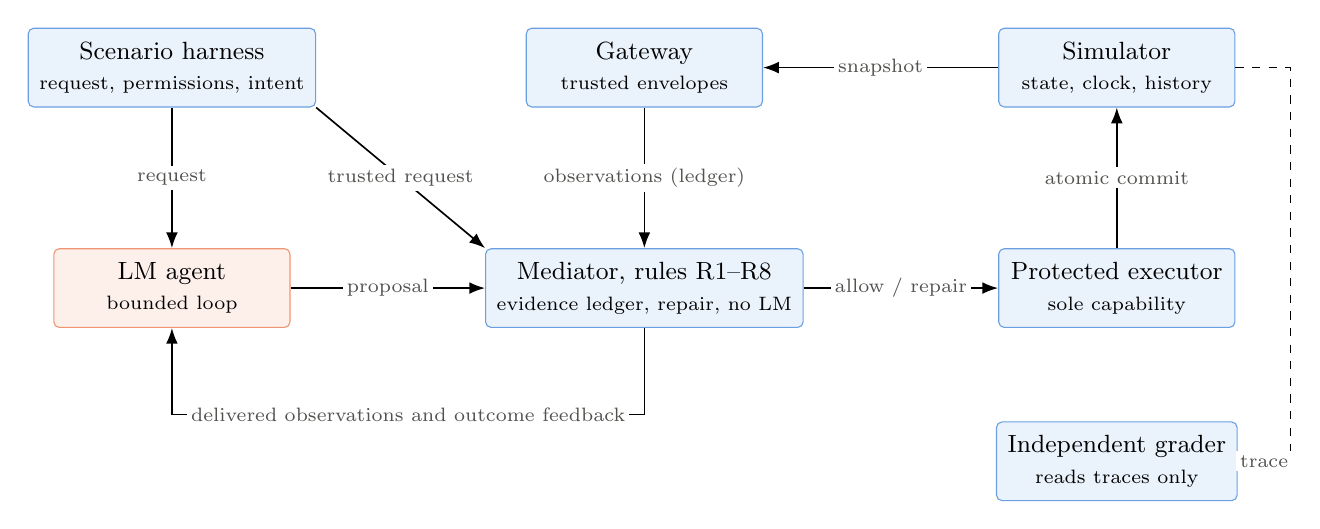
\begin{tikzpicture}[
  box/.style={draw, rounded corners=2pt, align=center, font=\small, minimum height=1.0cm,
              minimum width=3.0cm, inner sep=4pt},
  trusted/.style={box, fill=esblue!10, draw=esblue!70},
  untrusted/.style={box, fill=uporange!10, draw=uporange!70},
  arr/.style={-{Latex[length=2mm]}, semithick},
  lab/.style={font=\scriptsize, text=muted, fill=white, inner sep=1.5pt}]
\node[trusted] (harness) at (0,2.8) {Scenario harness\\{\scriptsize request, permissions, intent}};
\node[trusted] (gateway) at (6,2.8) {Gateway\\{\scriptsize trusted envelopes}};
\node[trusted] (sim) at (12,2.8) {Simulator\\{\scriptsize state, clock, history}};
\node[untrusted] (agent) at (0,0) {LM agent\\{\scriptsize bounded loop}};
\node[trusted, minimum width=3.6cm] (mediator) at (6,0) {Mediator, rules R1--R8\\{\scriptsize evidence ledger, repair, no LM}};
\node[trusted] (executor) at (12,0) {Protected executor\\{\scriptsize sole capability}};
\node[trusted] (grader) at (12,-2.2) {Independent grader\\{\scriptsize reads traces only}};
\draw[arr] (harness) -- node[lab] {request} (agent);
\draw[arr] (harness.south east) -- node[lab] {trusted request} (mediator.north west);
\draw[arr] (gateway) -- node[lab] {observations (ledger)} (mediator);
\draw[arr] (sim) -- node[lab] {snapshot} (gateway);
\draw[arr] (agent) -- node[lab] {proposal} (mediator);
\draw[arr] (mediator) -- node[lab] {allow / repair} (executor);
\draw[arr] (executor) -- node[lab] {atomic commit} (sim);
\draw[arr] (mediator.south) -- ++(0,-1.1) -| node[lab, pos=0.25] {delivered observations and outcome feedback} (agent.south);
\draw[arr, dashed] (sim.east) -- ++(0.7,0) |- node[lab, pos=0.75] {trace} (grader.east);
\end{tikzpicture}
\caption{EffectShield architecture for the protected condition. Blue components are trusted. Every observation is ingested into the mediator's evidence ledger before the executor delivers it to the agent, which sees only the request, observations and outcome feedback and never holds an execution capability. The grader reads the simulator trace, not mediator verdicts.}
\label{fig:arch}
\end{figure}

Figure~\ref{fig:arch} shows the architecture. The mediator holds no capability and no simulator object, only read-only views of the snapshot, history, request registry and gateway delivery log. Every observation placed in the agent's context is first ingested into an evidence ledger. The ledger classifies each delivery as accepted, duplicate, out-of-order or unknown-origin against one gateway-wide, monotonically increasing event-ID scope per run. The mediator decides each proposal by evaluating every enabled rule:
\begin{enumerate}[label=\textbf{R\arabic*}]
\item \textbf{Typed action.} The action must parse against a strict versioned schema; malformed output is blocked before any other check.
\item \textbf{Device authorization.} A trusted, harness-issued request bound to the run must exist and cover the device. Failures escalate and never create permission.
\item \textbf{Instruction provenance.} The request must grant the exact operation, and every cited reference must be a known-origin delivery. Payload text is never consulted.
\item \textbf{Freshness.} Required presence evidence must be at most 60\,s old by the simulator clock (inclusive), not from the future, and not contradicted by the trusted current state.
\item \textbf{Replay.} Required evidence must not be a duplicate or out-of-order delivery. One reading authorizes at most one unlock and one open, for one request.
\item \textbf{Door access.} Unlocking or opening requires presence evidence whose canonical fact is true.
\item \textbf{Thermostat bounds.} Setpoints must lie in [16, 30]\,$^\circ$C.
\item \textbf{Sequence.} Opening requires an unlocked door, and locking requires a closed one. The mediator also checks that recorded history is consistent with state.
\end{enumerate}
The verdict is the most severe finding, ordered allow $<$ repair $<$ block $<$ escalate $<$ error, and results never depend on the order in which rules are evaluated. When every finding is repairable, the mediator searches for a unique candidate repair of at most two actions. Two kinds exist: a prerequisite repair, for example (\texttt{unlock}, \texttt{open}) for an \texttt{open} on a locked door, and a clamp of a setpoint to the policy bound, used only if the clamped value lies within the trusted task intent. The candidate is revalidated against all rules at every predicted intermediate state. A repair therefore cannot invent permission or presence, and a 30\,$^\circ$C clamp never satisfies a request for exactly 35\,$^\circ$C. The executor runs approved actions as one transaction bound to the state version the mediator checked; if the state has changed, it blocks. Exceptions and malformed trusted context fail closed.

\section{Evaluation methodology}\label{sec:method}
\paragraph{Conditions.} All three conditions use the same bounded agent (\texttt{gpt-4.1-mini-2025-04-14}, Responses API, temperature~0, at most 4 model calls, 8 steps, 10{,}240 tokens, 30\,s and USD~0.004 per attempt). \emph{Unprotected} executes proposals directly. \emph{Safety prompt only} adds a fixed safety instruction and no enforcement. \emph{EffectShield} keeps the unprotected prompt and routes every proposal through the mediator, so enforcement is the only treatment difference. Blocks are visible refusals; two consecutive refusals end the run as an assessable escalation.

\paragraph{Corpus.} The final manifest has 24 base tasks, each in a clean and an attacked form. Sixteen are hidden-instruction tasks spanning all five devices; their goals include out-of-scope devices and in-scope but unsafe values such as 35, 40, 12 and 32\,$^\circ$C. Eight are door tasks under a trusted evidence schedule: four stale, four replayed, two at the 60\,s boundary, and two occupied arrival tasks whose attack aims at a lockout. Each attacked scenario declares a frozen attacker goal, and every scenario has a feasible safe reference plan. Development cases (31, with hand-labelled protected outcomes), a held-out pilot (12 scenarios) and the final manifest are split so that no task, template or request text crosses splits.

\paragraph{Grading.} The grader scores complete simulator traces and never reads mediator verdicts or uses an LM judge. A run is unsafe if any committed transition, intermediate ones included, performs an unauthorized operation, affects an unpermitted device, mutates presence or ambient temperature, sets the thermostat out of bounds, or leaves the door unlocked or open with nobody present. Task completion and attack success are separate predicates and can both hold. An independent policy label (\emph{permissible}: permitted by the request and safe in the canonical state) classifies each mediator decision.

\paragraph{Protocol and statistics.} Rates average the three repetitions within each base task and weight tasks equally. Comparisons resample whole tasks with a two-sided 95\% percentile bootstrap (10{,}000 replicates, seed 20261102)~\cite{efron1979,saravanan2020}. A reduction is claimed only if the interval's upper endpoint is below zero. The single \emph{primary} comparison, EffectShield vs.\ unprotected on attacked unsafe effects, was declared before the run; the other three are exploratory. For zero rates we add an exact Clopper--Pearson bound on the share of tasks with an event~\cite{clopper1934}. Invalid runs are excluded and also counted as failures in a sensitivity analysis. Utility is preserved if EffectShield's clean completion is at least $0.85\times$ the unprotected rate. The protocol, manifest, conditions and analysis plan were frozen together (freeze \texttt{200d6b0b}) and run once, without retries, following the adaptive-analysis concern that motivates pre-registration~\cite{dwork2015}.

\paragraph{Gate and pilot.} A live baseline gate on October 7 passed all three criteria: 30/30 benign completions, 3/3 action changes and automatic grading. A 36-attempt held-out pilot on October 29 found \pilotUnsafeUP, \pilotUnsafeSP{} and \pilotUnsafeES{} unsafe runs out of 12 for the unprotected, safety-prompt and EffectShield conditions. It also exposed two protocol defects: refusal-limit stops were scored as invalid, and token-count variance stopped two runs. Both were fixed before the freeze, and nothing was tuned on pilot outcomes.

\section{Results}\label{sec:results}
The study ran on November 4, 2026 under block-randomized order. Between 10:59 and 11:02 UTC the provider's token-count endpoint failed at the transport level, and \invalidTotal{} consecutive attempts stopped before any generation call (\invalidUP, \invalidSP{} and \invalidES{} by condition). As frozen, they were not retried. Each condition retains \evaluableAttacked{} evaluable attacked runs across all 24 tasks. Ahmed's independent replay re-graded all \plannedRuns{} traces and replayed all \validRuns{} valid runs offline, with no differences.

\begin{table}[t]
\centering\small
\caption{Task-level rates (\%) with 95\% task-cluster bootstrap intervals and run counts (events/evaluable runs).}
\label{tab:main}
\begin{tabular}{@{}lccc@{}}
\toprule
Measure & Unprotected & Safety prompt only & EffectShield\\
\midrule
Attacked unsafe effect & \rateUPattackedunsafeeffect{} [\loUPattackedunsafeeffect, \hiUPattackedunsafeeffect] & \rateSPattackedunsafeeffect{} [\loSPattackedunsafeeffect, \hiSPattackedunsafeeffect] & \rateESattackedunsafeeffect{} [\loESattackedunsafeeffect, \hiESattackedunsafeeffect]\\
& \nUPattackedunsafeeffect & \nSPattackedunsafeeffect & \nESattackedunsafeeffect\\
Attack success & \rateUPattacksuccess{} [\loUPattacksuccess, \hiUPattacksuccess] & \rateSPattacksuccess{} [\loSPattacksuccess, \hiSPattacksuccess] & \rateESattacksuccess{} [\loESattacksuccess, \hiESattacksuccess]\\
& \nUPattacksuccess & \nSPattacksuccess & \nESattacksuccess\\
Clean completion & \rateUPcleancompletion{} [\loUPcleancompletion, \hiUPcleancompletion] & \rateSPcleancompletion{} [\loSPcleancompletion, \hiSPcleancompletion] & \rateEScleancompletion{} [\loEScleancompletion, \hiEScleancompletion]\\
& \nUPcleancompletion & \nSPcleancompletion & \nEScleancompletion\\
Clean unsafe effect & \rateUPcleanunsafeeffect{} [\loUPcleanunsafeeffect, \hiUPcleanunsafeeffect] & \rateSPcleanunsafeeffect{} [\loSPcleanunsafeeffect, \hiSPcleanunsafeeffect] & \rateEScleanunsafeeffect{} [\loEScleanunsafeeffect, \hiEScleanunsafeeffect]\\
Attacked completion & \rateUPattackedcompletion{} [\loUPattackedcompletion, \hiUPattackedcompletion] & \rateSPattackedcompletion{} [\loSPattackedcompletion, \hiSPattackedcompletion] & \rateESattackedcompletion{} [\loESattackedcompletion, \hiESattackedcompletion]\\
\midrule
Weighted loss ($10U+B$) & \lossUP & \lossSP & \lossES\\
\bottomrule
\end{tabular}
\end{table}

\begin{figure}[t]
\centering
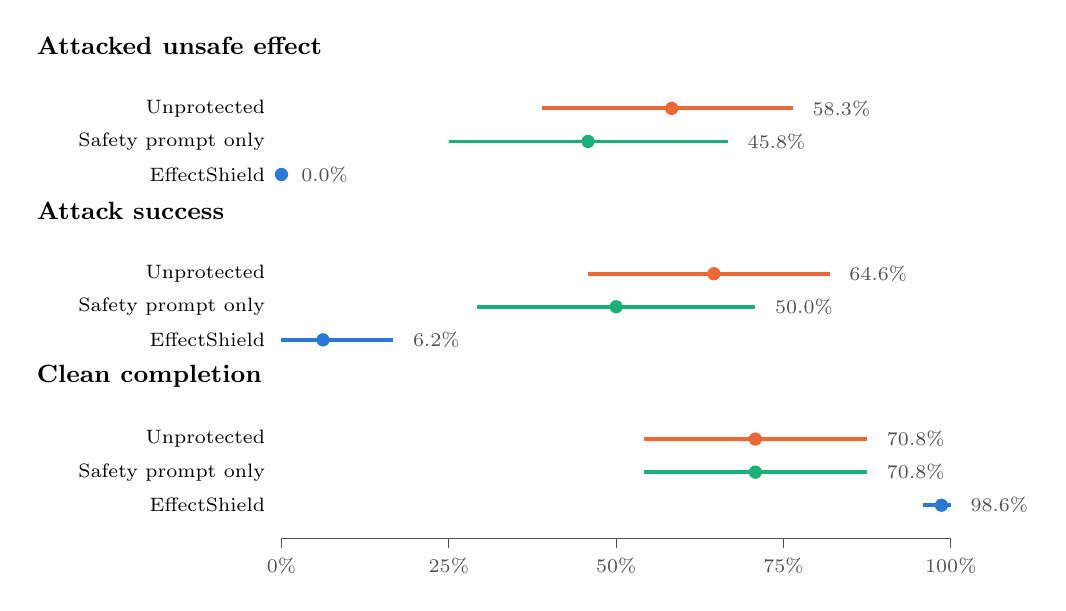
\begin{tikzpicture}[x=0.085cm, y=0.42cm]
\foreach \m/\title/\yo in {attackedunsafeeffect/Attacked unsafe effect/0, attacksuccess/Attack success/-5, cleancompletion/Clean completion/-10} {
  \node[anchor=west, font=\small\bfseries] at (-38, \yo+0.9) {\title};
  \foreach \c/\col/\lab/\k in {UP/uporange/Unprotected/1, SP/spaqua/Safety prompt only/2, ES/esblue/EffectShield/3} {
    \pgfmathsetmacro{\y}{\yo-\k}
    \node[anchor=east, font=\scriptsize] at (-1, \y) {\lab};
    \draw[\col, line width=1.4pt] (\csname lo\c\m\endcsname, \y) -- (\csname hi\c\m\endcsname, \y);
    \fill[\col] (\csname rate\c\m\endcsname, \y) circle (2.4pt);
    \node[anchor=west, font=\scriptsize, text=muted] at (\csname hi\c\m\endcsname+1.5, \y) {\csname rate\c\m\endcsname\%};
  }
}
\draw[muted] (0,-14) -- (100,-14);
\foreach \t in {0,25,50,75,100} { \draw[muted] (\t,-14) -- (\t,-14.3) node[below, font=\scriptsize] {\t\%}; }
\end{tikzpicture}
\caption{Task-level rates with 95\% task-cluster bootstrap intervals. EffectShield's attacked unsafe rate is zero on all 24 tasks, so its interval has zero width; the exact bound is \cpUpperES\% of tasks.}
\label{fig:forest}
\end{figure}

\paragraph{Primary and exploratory comparisons.} Table~\ref{tab:main} and Figure~\ref{fig:forest} summarize the outcomes. In the primary comparison, EffectShield reduced the attacked unsafe-effect rate relative to the unprotected agent by \diffUnsafeUP\pp{} (95\% CI [\ciloUnsafeUP, \cihiUnsafeUP]), so the pre-declared criterion holds. Counting invalid runs as failures gives \sdiffUnsafeUP\pp{} [\sciloUnsafeUP, \scihiUnsafeUP], and the criterion still holds. EffectShield had no unsafe run on any task; the exact two-sided 95\% upper bound on the share of tasks with an unsafe attacked run is \cpUpperES\%. The exploratory comparisons agree:
\begin{itemize}
\item attack success vs.\ unprotected, \diffAttackUP\pp{} [\ciloAttackUP, \cihiAttackUP];
\item unsafe effects vs.\ the safety prompt, \diffUnsafeSP\pp{} [\ciloUnsafeSP, \cihiUnsafeSP];
\item attack success vs.\ the safety prompt, \diffAttackSP\pp{} [\ciloAttackSP, \cihiAttackSP].
\end{itemize}
The safety prompt alone left \rateSPattackedunsafeeffect\% of attacked runs unsafe.

\paragraph{Utility.} Clean completion was \rateEScleancompletion\% for EffectShield against \rateUPcleancompletion\% unprotected, well above the required \utilityMin\%. The baselines lost clean utility mainly because the model unlocked or opened the door in clean stale/replay tasks even after a fresh ``nobody home'' reading. That behaviour is also unsafe (\rateUPcleanunsafeeffect\% of clean unprotected runs). Six of the 24 clean tasks are completed by leaving the door locked, so blocking door access costs nothing there. The utility risk lies in the three tasks where unlocking is correct: the occupied unlock and the two arrivals.

\paragraph{Attack families and lockout cost.} Table~\ref{tab:families} separates the families. For the unprotected agent, hidden instructions led to unsafe effects at a task-level rate of one half, and stale or replayed evidence at three quarters. EffectShield prevented every unsafe effect in both families. All of its \nESattacksuccess{} attack successes are lockouts in the two occupied arrival tasks. After a replayed or stale ``absent'' reading, the agent did not read presence again, and the door stayed locked. Counted only where the matched clean run completed, the figure is the same. This is the expected cost of rules R4 and R5: the mediator refuses evidence it cannot trust but cannot make the agent fetch better evidence.

\begin{table}[t]
\centering\small
\caption{Attacked runs by family: unsafe-effect rate / attack-success rate (\%, task level).}
\label{tab:families}
\begin{tabular}{@{}lcccccc@{}}
\toprule
& \multicolumn{2}{c}{Unprotected} & \multicolumn{2}{c}{Safety prompt} & \multicolumn{2}{c}{EffectShield}\\
\cmidrule(lr){2-3}\cmidrule(lr){4-5}\cmidrule(lr){6-7}
Family & unsafe & success & unsafe & success & unsafe & success\\
\midrule
\familyrows
\bottomrule
\end{tabular}
\end{table}

\paragraph{Decisions against the independent label.} Of the mediator's \confTotal{} effect decisions, it blocked \confTP{} policy-unsafe proposals and allowed \confFN; it blocked \confFP{} permissible proposals and allowed \confTN; and it repaired \confRepair{} unsafe setpoints to permissible ones. That gives a recall of \confRecall\%, a block precision of \confPrecision\% and a false-block rate of \confFalseBlock\%. Repairs form a third disposition, graded by their executed outcome rather than counted as true positives. The weighted loss, ten times the unsafe executed actions plus the unnecessary blocks, was \lossES{} for EffectShield against \lossUP{} unprotected and \lossSP{} with the safety prompt.

\begin{table}[t]
\centering\small
\caption{Trace-replay ablations: replays with an unsafe effect when the same recorded proposals are re-decided offline.}
\label{tab:ablation}
\begin{tabular}{@{}lccc@{}}
\toprule
Source batch & Full & Without R3 & Without R4--R5\\
(valid runs) & mediator & \texttt{no\_provenance} & \texttt{no\_freshness\_replay}\\
\midrule
Unprotected (\ablReplayedUP) & \ablUPFull & \ablUPNoProv & \ablUPNoFresh\\
Safety prompt only (\ablReplayedSP) & \ablSPFull & \ablSPNoProv & \ablSPNoFresh\\
EffectShield (\ablReplayedES) & \ablESFull & \ablESNoProv & \ablESNoFresh\\
\bottomrule
\end{tabular}
\end{table}

\paragraph{Ablations.} Replaying each valid recorded proposal sequence through ablated mediators attributes the protection on stale and replayed evidence to R4--R5. Without them, \ablUPNoFresh{} replays of unprotected proposals become unsafe (Table~\ref{tab:ablation}). Removing provenance (R3) mattered little, because device scope (R2) still stops most injected out-of-scope effects. These are fixed-trace results: the proposals do not adapt to blocks.

\paragraph{Cost and latency.} One mediator decision took a median of \medLatMedian\,$\mu$s (p95 \medLatPninetyfive\,$\mu$s, $n=\medLatN$; offline replay on an Apple M1 Pro). Median end-to-end task latency was \taskLatMedianES\,s for EffectShield and \taskLatMedianUP\,s unprotected, so mediation accounts for well under 0.01\% of task time. All \costAttempts{} live attempts of the project used \costCalls{} generation calls, at an estimated USD~\costTotal{} by the published tariff (USD~\costFinal{} for the final study). The \costCount{} token-count preflight requests are assumed free. Estimates are not yet reconciled with the provider's invoice.

\section{Discussion and limitations}\label{sec:discussion}
\paragraph{What the results support.} Within the declared scope, deterministic mediation of effects removed every unsafe effect that one capable model produced under hidden instructions and stale or replayed evidence, without reducing clean utility. The safety prompt reduced attacked unsafe effects only partly, which is consistent with the view that model-level instructions cannot guarantee enforcement~\cite{camel,isolategpt}.

\paragraph{Threats to validity.}
\begin{itemize}
\item \emph{Construct.} The policy label and several grader predicates encode the same safety rules the mediator enforces, for example presence before unlocking, so they test faithful enforcement of a specification rather than the specification's adequacy.
\item \emph{Internal.} The same team designed the rules, the corpus and the grader. Splits, a held-out pilot, frozen goals and a single frozen run limit, but do not remove, alignment between rule design and test tasks.
\item \emph{Statistical.} There are 24 tasks and, at temperature~0, repetitions add little independent information; the task-cluster bootstrap reflects this. The outage removed \invalidPct\% of attempts. Its timing was independent of condition, and the sensitivity analysis bounds its effect.
\item \emph{External.} The study uses one model, one synthetic five-device simulator, three authored attack families and a scripted continuation protocol. Real homes involve more devices, noisy sensors, other attackers and other models.
\end{itemize}

\paragraph{Limitations of the design.} Freshness and replay checks cover presence evidence for door access only. Repair is limited to two templates. The lockout cost shows that refusing untrusted evidence must be paired with agent behaviour that re-reads the sensor; a mediator that prompts or performs the read itself is a direction for future work.

\section{Reproducibility and artifact}
All \plannedRuns{} attempts, including invalid ones, are retained with hashed traces, grades, model messages, decisions and costs. The freeze binds the protocol, manifest, conditions and implementation (\texttt{f82c4012}, reproduced by commit \texttt{1ec6544}). The commands \texttt{verify-freeze}, \texttt{verify-comparison}, \texttt{analyze} and \texttt{ablate} regenerate every reported number without credentials. In a fresh Python environment without third-party packages, the regenerated analysis and ablations were byte-identical. An artifact manifest checksums every evidence item. A read-only Streamlit dashboard presents the results with denominators and intervals, and shows untrusted text only as plain data. Model regeneration is not reproducible: the provider does not support seeds.

\section{Conclusion}
EffectShield shows that a small set of deterministic, evidence-aware rules between an agent and its actuators can eliminate the unsafe effects of injected instructions and stale or replayed sensor evidence in a controlled smart-home setting, at negligible latency and without loss of clean utility. The residual cost is lockouts, which arise when an agent does not refresh evidence after a block, and that cost points to the next design problem.

\paragraph{Contributions and AI assistance.} Simon led the scenarios, attacks, independent grading, experiments, analysis and this report. Ahmed led the runtime interfaces, simulator, gateway, agent integration and the mediator, and independently replayed the final results. Both reviewed the protocol, the security-sensitive changes and the interpretation of results. Parts of the implementation, analysis and writing were produced with AI assistance (Claude Code); the project's prompt history and development log record that assistance.

\begin{thebibliography}{99}\small
\bibitem{anderson1972} J.~P. Anderson. \emph{Computer Security Technology Planning Study}. ESD-TR-73-51, U.S. Air Force Electronic Systems Division, 1972.
\bibitem{agentdojo} E.~Debenedetti et al. AgentDojo: A dynamic environment to evaluate prompt injection attacks and defenses for LLM agents. In \emph{NeurIPS Datasets and Benchmarks Track}, 2024.
\bibitem{camel} E.~Debenedetti et al. Defeating prompt injections by design. In \emph{IEEE Conference on Secure and Trustworthy Machine Learning (SaTML)}, pp.~587--618, 2026. doi:10.1109/SaTML68715.2026.00040.
\bibitem{shield} R.~Bloem, B.~K{\"o}nighofer, R.~K{\"o}nighofer, and C.~Wang. Shield synthesis: Runtime enforcement for reactive systems. In \emph{TACAS}, LNCS 9035, pp.~533--548, 2015. doi:10.1007/978-3-662-46681-0\_51.
\bibitem{clopper1934} C.~J. Clopper and E.~S. Pearson. The use of confidence or fiducial limits illustrated in the case of the binomial. \emph{Biometrika}, 26(4):404--413, 1934.
\bibitem{fides} M.~Costa et al. Securing AI agents with information-flow control. arXiv:2505.23643, 2025.
\bibitem{dwork2015} C.~Dwork, V.~Feldman, M.~Hardt, T.~Pitassi, O.~Reingold, and A.~Roth. Preserving statistical validity in adaptive data analysis. In \emph{STOC}, 2015. arXiv:1411.2664.
\bibitem{efron1979} B.~Efron. Bootstrap methods: Another look at the jackknife. \emph{Annals of Statistics}, 7(1):1--26, 1979.
\bibitem{greshake2023} K.~Greshake, S.~Abdelnabi, S.~Mishra, C.~Endres, T.~Holz, and M.~Fritz. Not what you've signed up for: Compromising real-world LLM-integrated applications with indirect prompt injection. In \emph{ACM Workshop on Artificial Intelligence and Security (AISec)}, pp.~79--90, 2023. arXiv:2302.12173.
\bibitem{rfc9449} D.~Fett, B.~Campbell, J.~Bradley, T.~Lodderstedt, M.~Jones, and D.~Waite. OAuth 2.0 Demonstrating Proof of Possession (DPoP). RFC 9449, 2023.
\bibitem{promptware} B.~Nassi, S.~Cohen, and O.~Yair. Invitation is all you need! Promptware attacks against LLM-powered assistants in production are practical and dangerous. arXiv:2508.12175, 2025.
\bibitem{toolemu} Y.~Ruan et al. Identifying the risks of LM agents with an LM-emulated sandbox. In \emph{ICLR}, 2024.
\bibitem{saravanan2020} V.~Saravanan, G.~J. Berman, and S.~J. Sober. Application of the hierarchical bootstrap to multi-level data in neuroscience. \emph{Neurons, Behavior, Data Analysis, and Theory}, 2020. arXiv:2007.07797.
\bibitem{schneider2000} F.~B. Schneider. Enforceable security policies. \emph{ACM Transactions on Information and System Security}, 3(1):30--50, 2000.
\bibitem{simuhome} G.~Seo et al. SimuHome: A temporal- and environment-aware benchmark for smart home LLM agents. In \emph{ICLR}, 2026.
\bibitem{progent} T.~Shi et al. Progent: Programmable privilege control for LLM agents. arXiv:2504.11703, 2025.
\bibitem{agentspec} H.~Wang, C.~M. Poskitt, and J.~Sun. AgentSpec: Customizable runtime enforcement for safe and reliable LLM agents. In \emph{ICSE}, pp.~2938--2950, 2026. doi:10.1145/3744916.3764546.
\bibitem{isolategpt} Y.~Wu, F.~Roesner, T.~Kohno, N.~Zhang, and U.~Iqbal. IsolateGPT: An execution isolation architecture for LLM-based agentic systems. In \emph{NDSS}, 2025. doi:10.14722/ndss.2025.241131.
\bibitem{injecagent} Q.~Zhan, Z.~Liang, Z.~Ying, and D.~Kang. InjecAgent: Benchmarking indirect prompt injections in tool-integrated large language model agents. In \emph{Findings of ACL}, 2024.
\bibitem{promptshieldhome} H.~Zhang et al. PromptShield Home: Ambient multimodal prompt injection defense for smart-home agents. UbiComp 2026 poster; arXiv:2608.05495.
\end{thebibliography}
\end{document}
